\section{Evaluation}
\label{sec:evaluation}
Our system needs be suitable for economical use. We can express this as two requirements: On the one hand, the found combined NER and EL process should find as many correct references to organizations as possible. While Ehmüller~\cite{ehmueller} evaluates this in terms of the standard measures precision, recall and $F_1$ score, this thesis focuses on how significant the features are without considering a certain classifier model. On the other hand, our system has to be capable of processing large amounts of data in reasonable time. As our project aims at solving this using cluster computing, this evaluation considers how well the described preprocessing scales out.



\subsection{Significance of the features}
Given an entity $en$ and a link candidate $lc=(a_{lc}, c_{lc})$ consisting of an alias $a_{lc}$ and its context $c_{lc}$, the classifier decides whether $lc$ references $en$ or not. Note that, while the link candidate's entity score $es_{en}(a_{lc})$ and the context score $cs_{en}(c_{lc})$ depend on $en$, the link score $ls(a_{lc})$ only depends on the alias itself. Therefore these features must allow a distinction between valid and invalid links regarding the given entity. The following paragraphs evaluate the distribution of the features based on a sample of exactly 100,000 composite features from our training data and how expressive they are for this distinction.

\begin{figure}[ht]
	\begin{tabular}{cc}
	\subfloat[Composite distribution of the entity score and the context score]{
		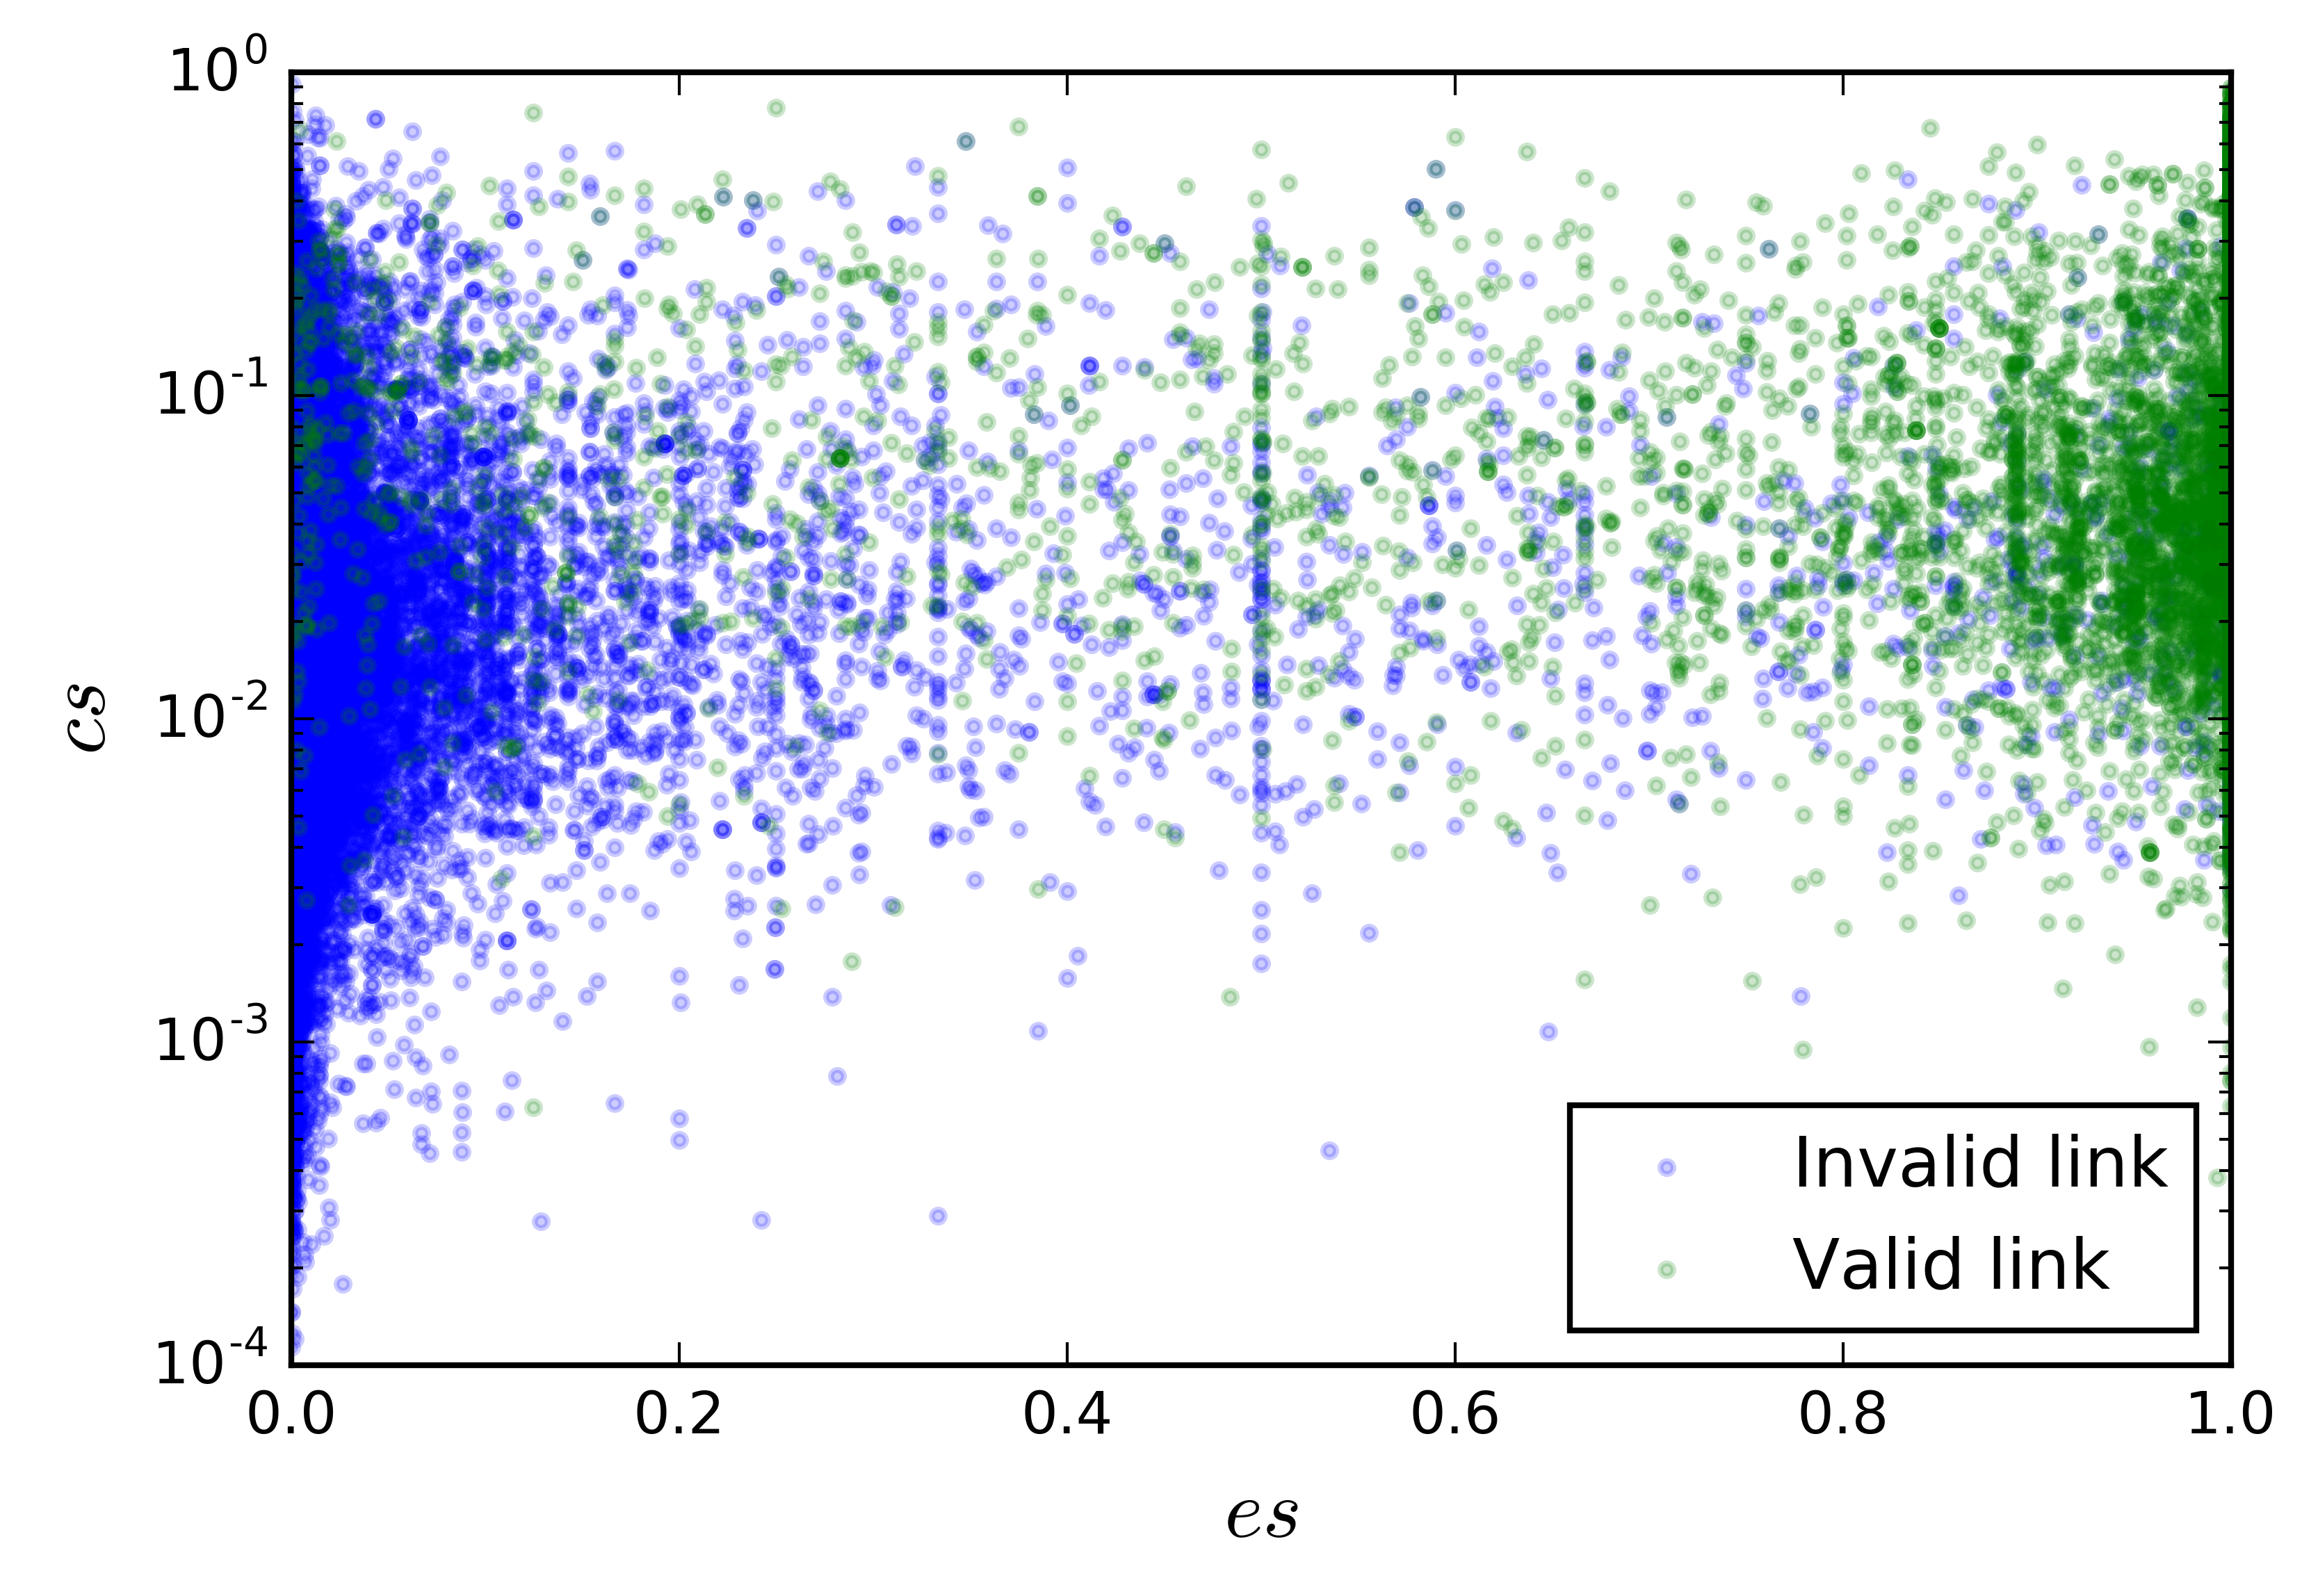
\includegraphics[width = 0.45\textwidth]{Graphics/feature_evaluation/composite_features.png}
		\label{fig:composite_features}
	} &
	\subfloat[Distribution of the link scores]{
		\includegraphics[width = 0.45\textwidth]{Graphics/feature_evaluation/link_scores.pdf}
		\label{fig:link_scores}
	}\\
	\subfloat[Distribution of the entity scores]{
		\includegraphics[width = 0.45\textwidth]{Graphics/feature_evaluation/entity_scores.pdf}
		\label{fig:entity_scores}
	} &
	\subfloat[Distribution of the context scores]{
		\includegraphics[width = 0.45\textwidth]{Graphics/feature_evaluation/context_scores.pdf}
		\label{fig:context_scores}
	}
	\end{tabular}
	\caption{The link score, entity score and context score have significantly different distributions for valid and invalid links.}
	\label{fig:distributions}
\end{figure}

Figure~\ref{fig:composite_features} gives an overview of the composite distribution of the entity score and context score. Note that the context score is scaled logarithmically. The diagram reveals three properties:

\begin{enumerate}
\item There are two clearly identifiable \textbf{clusters}: One for valid links and a high entity score and one for invalid links and a small entity score. 

\item The entity score is \textbf{more expressive} than the context score, as the clusters can only be separated using the entity score.

\item There is a \textbf{correlation} between the entity score and the context score: The upper right half of the diagram contains a lot more valid links than its lower left half. This means that the entity score and context score are "confirming" each other.
\end{enumerate}

Now we consider the features separately to get a more concise understanding of their quality:

\paragraph{Link score}
Figure~\ref{fig:link_scores} shows the distribution of the link scores for the valid and invalid links. Here and in the following, the overlap between the bars is shaded in dark blue. As not more than one entity is valid for each link candidate, our sample contains only 8.4\% valid links. Thus, for the better visibility, $f$ shows the relative frequency of the link scores. It is 1 both for the valid and invalid links if added up. We can see that a valid link has a link score that is close to 1 in more than 60\% of cases, while invalid links have a link score that is widely distributed. In fact, almost all of the links represented by the last bar have a link score, which is exactly 1. This means that there are a lot of explicit aliases, which always refer to the same entities. 

\paragraph{Entity score}
Figure~\ref{fig:entity_scores} shows the distribution of the entity scores. The extreme left and extreme right bar represent the clusters observed in Figure~\ref{fig:composite_features}. Hence the entity score is very expressive for our task. A classifier that decides based on a linear separation between these clusters should yield reasonable results. But since the of portion valid links is relatively small, this feature is not sufficient.

\paragraph{Context score}
Finally, Figure~\ref{fig:context_scores} shows the distribution of the context scores. Note that the frequency is scaled logarithmically. Although there is a large overlap between the valid and the invalid links, the distribution of the valid links is significantly shifted to greater context scores. For a context score of about 0.1, the context score has the least significance. The smaller or greater it becomes from there, the better the classifier can make its decisions.

\paragraph{Second order features}
Also the second order features have a high expressiveness, as shown in Figure~\ref{fig:second_order_features} in the appendix. Similar to the three features described above, they show significantly different distributions for valid and invalid links. Thanks to their support, the classifier improves the results of the EL even further.


\subsection{Scale out}
\begin{figure}[ht]
	\centering
  \includegraphics[width=\textwidth]{Graphics/CosineContextComparator.pdf}
	\caption{Scale out of the context score computation}
	\label{fig:scale_out}
\end{figure}

To make our system scalable for arbitrary input sizes, we use the cluster computing framework Apache Spark\footnotemark{}. Figure~\ref{fig:scale_out} shows the scale out of the context score computation for a sample of 100,000 Wikipedia articles. Starting from the bags of words, this comprises the calculation of the tf-idf vectors and its respective cosine similarities. The context score computation is one of our most time-consuming tasks.
\footnotetext{\url{https://spark.apache.org/}, last accessed on \formatdate{20}{7}{2017}.}

We have calculated the efficiency as the average amount of articles that is processed within a second and measured the scale out for a different number of nodes (i.e., physical computers), while the number or CPU cores was constant. For the better interpretation of the results, the diagram also depicts a linear scale out. It denotes that the efficiency increases in the same proportion as the number of nodes. Since there is always communication overhead between the nodes, which increases runtimes, a linear scale out or even super-linear scale out is difficult to achieve. As we can see, we reach a linear scale out for two nodes, but overall, the scale out is sub-linear. The smaller increase for more than two nodes might be explained by the relatively small input sample, which increases the proportion of the communication overhead. The other steps of our preprocessing show a similar scale out behavior.

To contextualize our approach, we compare the extraction of the bags of words and the subsequent tf-idf computation to another implementation for the same task. This implementation is part of the Spark MLlib\footnotemark{}, which was specially designed for cluster computing. 15 runs of both implementations for all links of the German Wikipedia led to an average time of 9.5 minutes for the Spark MLlib and 6.5 minutes for our approach. Therefore, it computes the contexts of link candidates 1.5 times faster than the Spark MLlib.
\footnotetext{\url{https://spark.apache.org/mllib/}, last accessed on \formatdate{20}{7}{2017}.}

~\\

As shown above, the features we use for the extraction of business relations from text have a high quality. They allow a distinction between valid and invalid references to entities. Furthermore, our preprocessing is suitable for cluster computing. It can be distributed over multiple nodes and has an increasing efficiency for a higher amount of computing resources.